%QUESTIONS HERE
%<*mytag1>
\begin{questions}[start=\number\value{questionsi}+1,noitemsep,leftmargin=20mm,labelsep=0.1cm]
\item What is the purpose of flashing the Access point with OpenWRT, rather than keeping DD-WRT?
\end{questions}
%</mytag1>

%<*mytag2>
\begin{questions}[resume,start=\number\value{questionsi}+1,noitemsep,leftmargin=20mm,labelsep=0.1cm]
\item What is 802.11s and why is it used?
\end{questions}
%</mytag2>

%<*mytag3>
\begin{questions}[resume,start=\number\value{questionsi}+1,noitemsep,leftmargin=20mm,labelsep=0.1cm]
\item On a machine with wireless capabilities, is the SSID of OpenWRTBabel1 visible?
\end{questions}
%</mytag3>

%<*mytag4>
\begin{questions}[resume,start=\number\value{questionsi}+1,noitemsep,leftmargin=20mm,labelsep=0.1cm]
\item What is the purpose of using uci to configure the router?
\end{questions}
%</mytag4> 

%<*mytag5>
\begin{questions}[resume*,start=\number\value{questionsi}+1,noitemsep,leftmargin=20mm,labelsep=0.1cm]
\item
\end{questions}
%</mytag5> 

%<*mytag6>
\begin{questions}[resume,start=\number\value{questionsi}+1,noitemsep,leftmargin=20mm,labelsep=0.1cm]
\item 
\item
\end{questions}
%</mytag6> 

%<*mytag7>
\begin{questions}[resume*,start=\number\value{questionsi}+1,noitemsep,leftmargin=20mm,labelsep=0.1cm]
\item 
\item
\end{questions}
%</mytag7>

%<*mytag8>
\begin{questions}[resume,start=\number\value{questionsi}+1,noitemsep,leftmargin=20mm,labelsep=0.1cm]
\item 
\item
\end{questions}
%</mytag8>

%<*mytag9>
\begin{questions}[resume,start=\number\value{questionsi}+1,noitemsep,leftmargin=20mm,labelsep=0.1cm]
\item 
\item
\end{questions}
%</mytag9>

%LISTS HERE

%<*mytag10>
\begin{enumerate}[noitemsep,label=$\circ$,leftmargin=17mm,labelsep=0.5cm]
\item
\item
\end{enumerate}
%</mytag10>

%<*mytag11>
\begin{enumerate}[noitemsep,leftmargin=10mm,labelsep=0.1cm]
\item Test item
\item
\end{enumerate}
%</mytag11>


%COMMANDS HERE
%<*mytag12>
\begin{enumerate}[noitemsep,leftmargin=10mm,labelsep=0.1cm]
\item [] \textbf{ssh root@192.168.10.1}  
\end{enumerate}
%</mytag12>

%<*mytag13>
\begin{enumerate}[noitemsep,leftmargin=10mm,labelsep=0.1cm]
\item [] \textbf{opkg install babeld kmod-ipv6}
\end{enumerate}
%</mytag13>
%<*mytag14>
\begin{enumerate}[noitemsep,label=$\circ$,leftmargin=17mm,labelsep=0.5cm]
\item [] \textbf{/etc/init.d/babeld enable}
\end{enumerate}
%</mytag14>
%<*mytag15>
\begin{enumerate}[noitemsep,leftmargin=10mm,labelsep=0.1cm]
\item [] \textbf{uci set network.wan=interface}
\item [] \textbf{uci set network.wan.ifname=wlan0}
\item [] \textbf{uci set network.wan.proto=static}
\item [] \textbf{uci set network.wan.ipaddr=192.168.10.1}
\item [] \textbf{uci set network.wan.netmask=255.255.255.255}
\end{enumerate}
%</mytag15>
%<*mytag16>
\begin{enumerate}[noitemsep,leftmargin=10mm,labelsep=0.1cm]
\item [] \textbf{opkg update}
\end{enumerate}
%</mytag16>
%<*mytag17>
\begin{enumerate}[noitemsep,leftmargin=10mm,labelsep=0.1cm]
\item [] \textbf{babeld -d1 br-lan}
\end{enumerate}
%</mytag17>
%<*mytag18>
\begin{enumerate}[noitemsep,leftmargin=10mm,labelsep=0.1cm]
\item [] \textbf{/etc/init.d/firewall reload}
\item [] \textbf{/etc/init.d/network reload}
\end{enumerate}
%</mytag18>
%<*mytag19>
\begin{enumerate}[noitemsep,leftmargin=10mm,labelsep=0.1cm]
\item [] \textbf{option mesh\_id "meshTest"}
\end{enumerate}
%</mytag19>
%<*mytag20>
\begin{enumerate}[noitemsep,leftmargin=10mm,labelsep=0.1cm]
\item [] \textbf{route -n}
\end{enumerate}
%</mytag20>
%<*mytag21>
\begin{enumerate}[noitemsep,leftmargin=10mm,labelsep=0.1cm]
\item [] \textbf{tcpdump -i br-lan -w babelTraffic.pcap}
\end{enumerate}
%</mytag21>
%<*mytag22>
\begin{enumerate}[noitemsep,leftmargin=10mm,labelsep=0.1cm]
\item [] \textbf{ps aux | grep tac\textunderscore plus} 
\end{enumerate}
%</mytag22>
%<*mytag23>
\begin{enumerate}[noitemsep,leftmargin=10mm,labelsep=0.1cm]
\item [] \textbf{netstat -an | grep :49}
\end{enumerate}
%</mytag23>
%<*mytag24>
\begin{enumerate}[noitemsep,leftmargin=10mm,labelsep=0.1cm]
\item [] \textbf{services}
\end{enumerate}
%</mytag24>
%<*mytag25>
\begin{enumerate}[noitemsep,leftmargin=10mm,labelsep=0.1cm]
\item [] \textbf{vulns}
\end{enumerate}
%</mytag25>
%<*mytag26>
\begin{enumerate}[noitemsep,leftmargin=10mm,labelsep=0.1cm]
\item [] \textbf{db\_import $<$name of the Nessus scan file including path$>$}
\end{enumerate}
%</mytag26>
%<*mytag27>
\begin{enumerate}[noitemsep,leftmargin=10mm,labelsep=0.1cm]
\item [] \textbf{vulns}
\end{enumerate}
%</mytag27>

%<*mytag28>
\begin{enumerate}[noitemsep,label=$\circ$,leftmargin=14mm,labelsep=0.5cm]
\item
\end{enumerate}
%</mytag28>


%GRAPHICS HERE

%<*mtag1>
\begin{figure}[H]
\centering
\captionsetup{width=.8\linewidth}
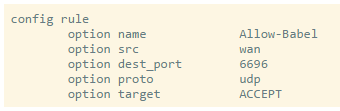
\includegraphics[scale=0.9]{img/configFirewall.png}
\caption{}
\label{fig:1}
\centering
\end{figure}
%</mtag1>

%<*mtag2>
\begin{figure}[H]
\centering
\captionsetup{width=.8\linewidth}
\includegraphics[scale=0.9]{img/.png}
\caption{}
\label{fig:2}
\centering
\end{figure}
%</mtag2>

%<*mtag3>
\begin{figure}[H]
\centering
\captionsetup{width=.8\linewidth}
\includegraphics[scale=0.9]{img/.png}
\caption{}
\label{fig:3}
\centering
\end{figure}
%</mtag3>